\documentclass[12pt]{article}

\usepackage{fullpage}
\usepackage{multicol,multirow}
\usepackage{tabularx}
\usepackage{ulem}
\usepackage{graphicx}%Вставка картинок правильная
\usepackage{float}%"Плавающие" картинки
\usepackage{wrapfig}%Обтекание фигур (таблиц, картинок и прочего)
\usepackage[utf8]{inputenc}
\usepackage[russian]{babel}

% Оригиналный шаблон: http://k806.ru/dalabs/da-report-template-2012.tex

\begin{document}

\section*{Лабораторная работа №\,2 по курсу дискрeтного анализа: словарь}

Выполнил студент группы 08-207 МАИ \textit{Дегтярев Денис Андреевич}.

\subsection*{Условие}

Необходимо создать программную библиотеку, реализующую
указанную структуру данных, на основе которой разработать
программу-словарь. В словаре каждому ключу, представляющему из
себя регистронезависимую последовательность букв английского
алфавита длиной не более 256 символов, поставлен в соответствие
некоторый номер, от 0 до $2^{64}$ - 1. Разным словам может быть
поставлен в соответствие один и тот же номер.  
Программа должна обрабатывать строки входного файла до его
окончания. Каждая строка может иметь следующий формат:  

\hspace{1 cm} \textbf{+ word 34} — добавить слово «word» с номером 34 в словарь. Программа должна вывести строку «OK», если операция прошла
успешно, «Exist», если слово уже находится в словаре.  

\hspace{1 cm} \textbf{- word} — удалить слово «word» из словаря. Программа должна
вывести «OK», если слово существовало и было удалено,
«NoSuchWord», если слово в словаре не было найдено.
word — найти в словаре слово «word». Программа должна вывести
«OK: 34», если слово было найдено; число, которое следует за
«OK:» — номер, присвоенный слову при добавлении. В случае,
если слово в словаре не было обнаружено, нужно вывести строку
«NoSuchWord».  

\hspace{1 cm} \textbf{! Save /path/to/file} — сохранить словарь в бинарном компактном
представлении на диск в файл, указанный параметром команды.
В случае успеха, программа должна вывести «OK», в случае
неудачи выполнения операции, программа должна вывести
описание ошибки (см. ниже).  

\hspace{1 cm} \textbf{! Load /path/to/file} — загрузить словарь из файла. Предполагается,
что файл был ранее подготовлен при помощи команды Save. В
случае успеха, программа должна вывести строку «OК», а
загруженный словарь должен заменить текущий (с которым
происходит работа); в случае неуспеха, должна быть выведена
диагностика, а рабочий словарь должен остаться без изменений.
Кроме системных ошибок, программа должна корректно
обрабатывать случаи несовпадения формата указанного файла и
представления данных словаря во внешнем файле.  

Для всех операций, в случае возникновения системной ошибки
(нехватка памяти, отсутствие прав на запись и т.п.), программа
должна вывести строку, начинающуюуся с «ERROR:» и описывающую
на английском языке возникшую ошибку.  

Структура данных: RB-дерево

\subsection*{Метод решения}

Реализовал данную структуру в виде класса. Каждую операцию(вставка, удаление и прочее) делал, 
как описывали на лекции.

\subsection*{Описание программы}

Insert(вставка элемента) - сначала выполняется как обычная вставка в бинарном дереве поиска
(цвет автоматически ставится красный), затем делается проверка на выполнение свойств дерева:  

1) Если отец черный - все норм.  

2) Если отец и дядя красный, то делаем их черными.  

3) Если отец красный, а дядя черный(долго описывать, проще и понятнее картинки):
\begin{figure*}[ht!]
    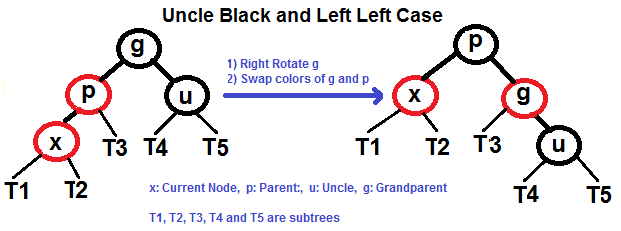
\includegraphics[height=5.5cm,width=.45\textwidth]{redBlackCase3a1.png}\hfill
    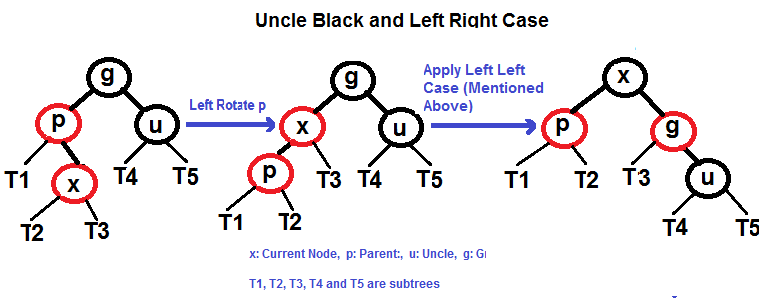
\includegraphics[height=5.5cm,width=.45\textwidth]{redBlackCase3b.png}
\end{figure*}
\begin{figure*}[ht!]
    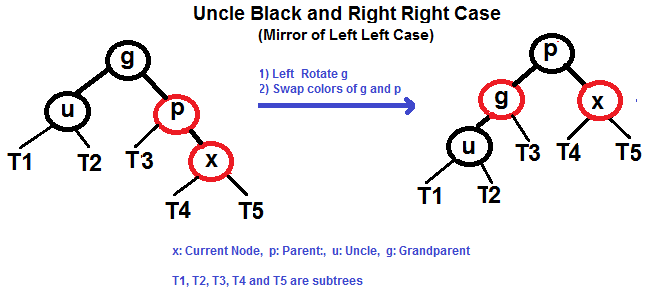
\includegraphics[height=5.5cm,width=.45\textwidth]{redBlackCase3c.png}\hfill
    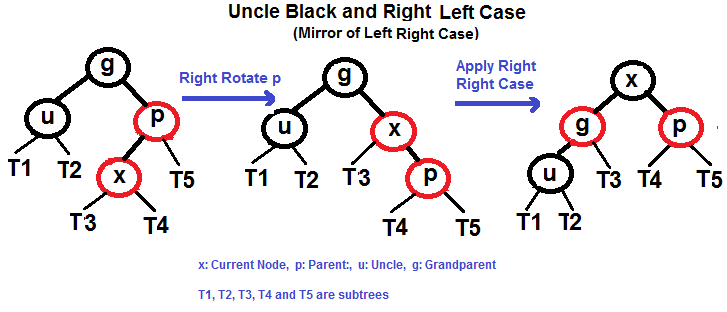
\includegraphics[height=5.5cm,width=.45\textwidth]{redBlackCase3d.png}
\end{figure*}

\noindent Все это выполняется пока цвет родителя красный. В конце на всякий случай корень перекрашивается
в черный.  

\noindent Search(поиск элемента) - такой же поиск как в бинарном дереве.  

\noindent Delete(удаление элемента) - тут три ситуации:  

1) 0 детей - удаляем.  

2) 1 ребенок - swap с ребенком значений и удаление ребенка.  

3) 2 детей - берем минимальный элемент правого ребенка, свапаем его с удаляемым элементом.  

\noindent Далее пока цвет искомой вершины черный выполняются те же действия, что и в Insert.

\noindent Save(дерево сохраняется в бинарный файл как словарь) - идет сохранение от корня, 1 элемент -
value, 2 элемент - цвет(0 - черный, 1 - красный), 3 элемент - левый сын, 4 элемент - правый сын. 
И так для каждого элемента.  

\noindent Load(дерево загружается из бинарного, предварительно сохраненного командой Save, файла) - реверс действий Save.  

\subsection*{Дневник отладки}

Первые посылки были сделаны до того, пока я не прочитал телегу(в случае ошибки записи в файл
или чтения из него выводил "OK"). Ошибка в 13 тесте - в конце массива char обязательно должен
быть \textbackslash0, иначе будут проблемы с выгрузкой этой строки с файла(вместо
char[256] нужно создавать массив char[257]).

\subsection*{Тест производительности}

\begin{figure*}[ht!]
    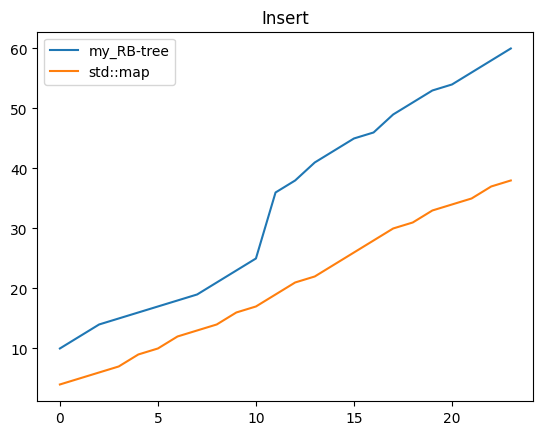
\includegraphics[height=6cm,width=.33\textwidth]{res_speed_add.png}\hfill
    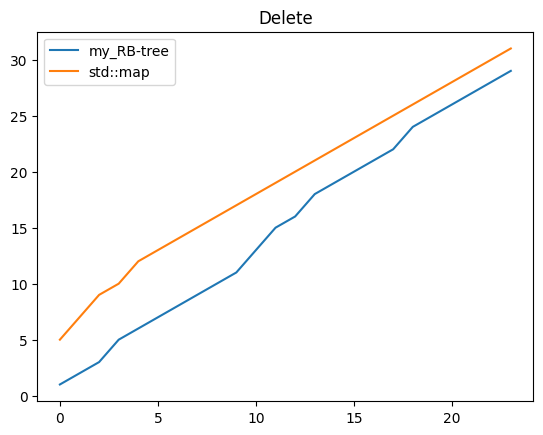
\includegraphics[height=6cm,width=.33\textwidth]{res_speed_del.png}\hfill
    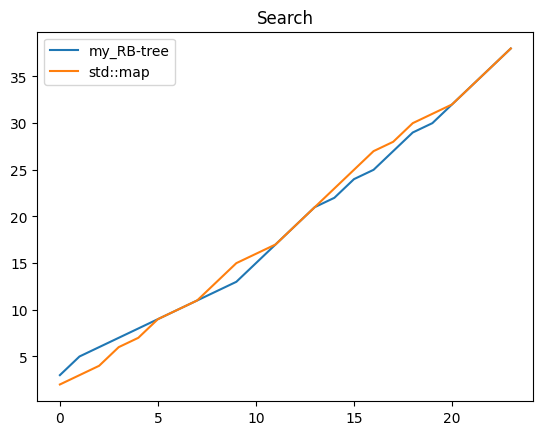
\includegraphics[height=6cm,width=.33\textwidth]{res_speed_search.png}
\end{figure*}

\subsection*{Недочёты}

Недочетов не должно быть... Реализовывал все добросовестно.

\subsection*{Выводы}

По графику видно, что RB-дерево работает за логарифмическое время. Это действительно полезно,
ведь для операции вставки за линейное время при большом кол-ве данных требуется очень много 
времени, а $log_2$(n) значительно ускоряет работу программы...

\end{document}
